\chapter{Seri Hat Hata Ayıklama Portu (Serial Wire Debug Port, SW-DP)}

\acrfull{SWD}, iki pin bağlantısı ile, JTAG arayüzüne alternatif olarak, pin kısıtlaması olan mikrodenetleyiciler için geliştirilmiştir.
ARM Hata Ayıklama Arayüzü v5 [1] ile tanımlanmış olan SWD, hata ayıklma portu ile ARM işlmecisinin \acrshort{AMBA} veriyoluna erişim sağlar. Bu sayade
işlmecinin sistem hafıza birimlerine, çevre birimlerinin ve sistem yazmaçlarına erişim sağlamaktadır.

\acrfull{DAP}, Hata Ayıklma Portu (\acrshort{DP}) ve Erişim Portu (\acrshort{AP}) olmak üzere iki ana kontrol birimine arılmıştır. ARM işlemcisine erişmek isteyen cihaz
Seri Hat Hata Ayıklama Portu'nun SWDIO ve SCLK pinlerine fiziksel olarak bağlanması gerekmektedir. SWD-DP ile sistemin geri kalan erişim ve hata ayıklama portuna erişim
sağlamak mümkündür. \acrfull{MEM-AP}, dahili AHB/APB veriyollarına, hafıza elemanlarına ve çevre birimlerine erişim sağlayabilen en önemli erişim portudur.

\begin{figure}[h]
\centering
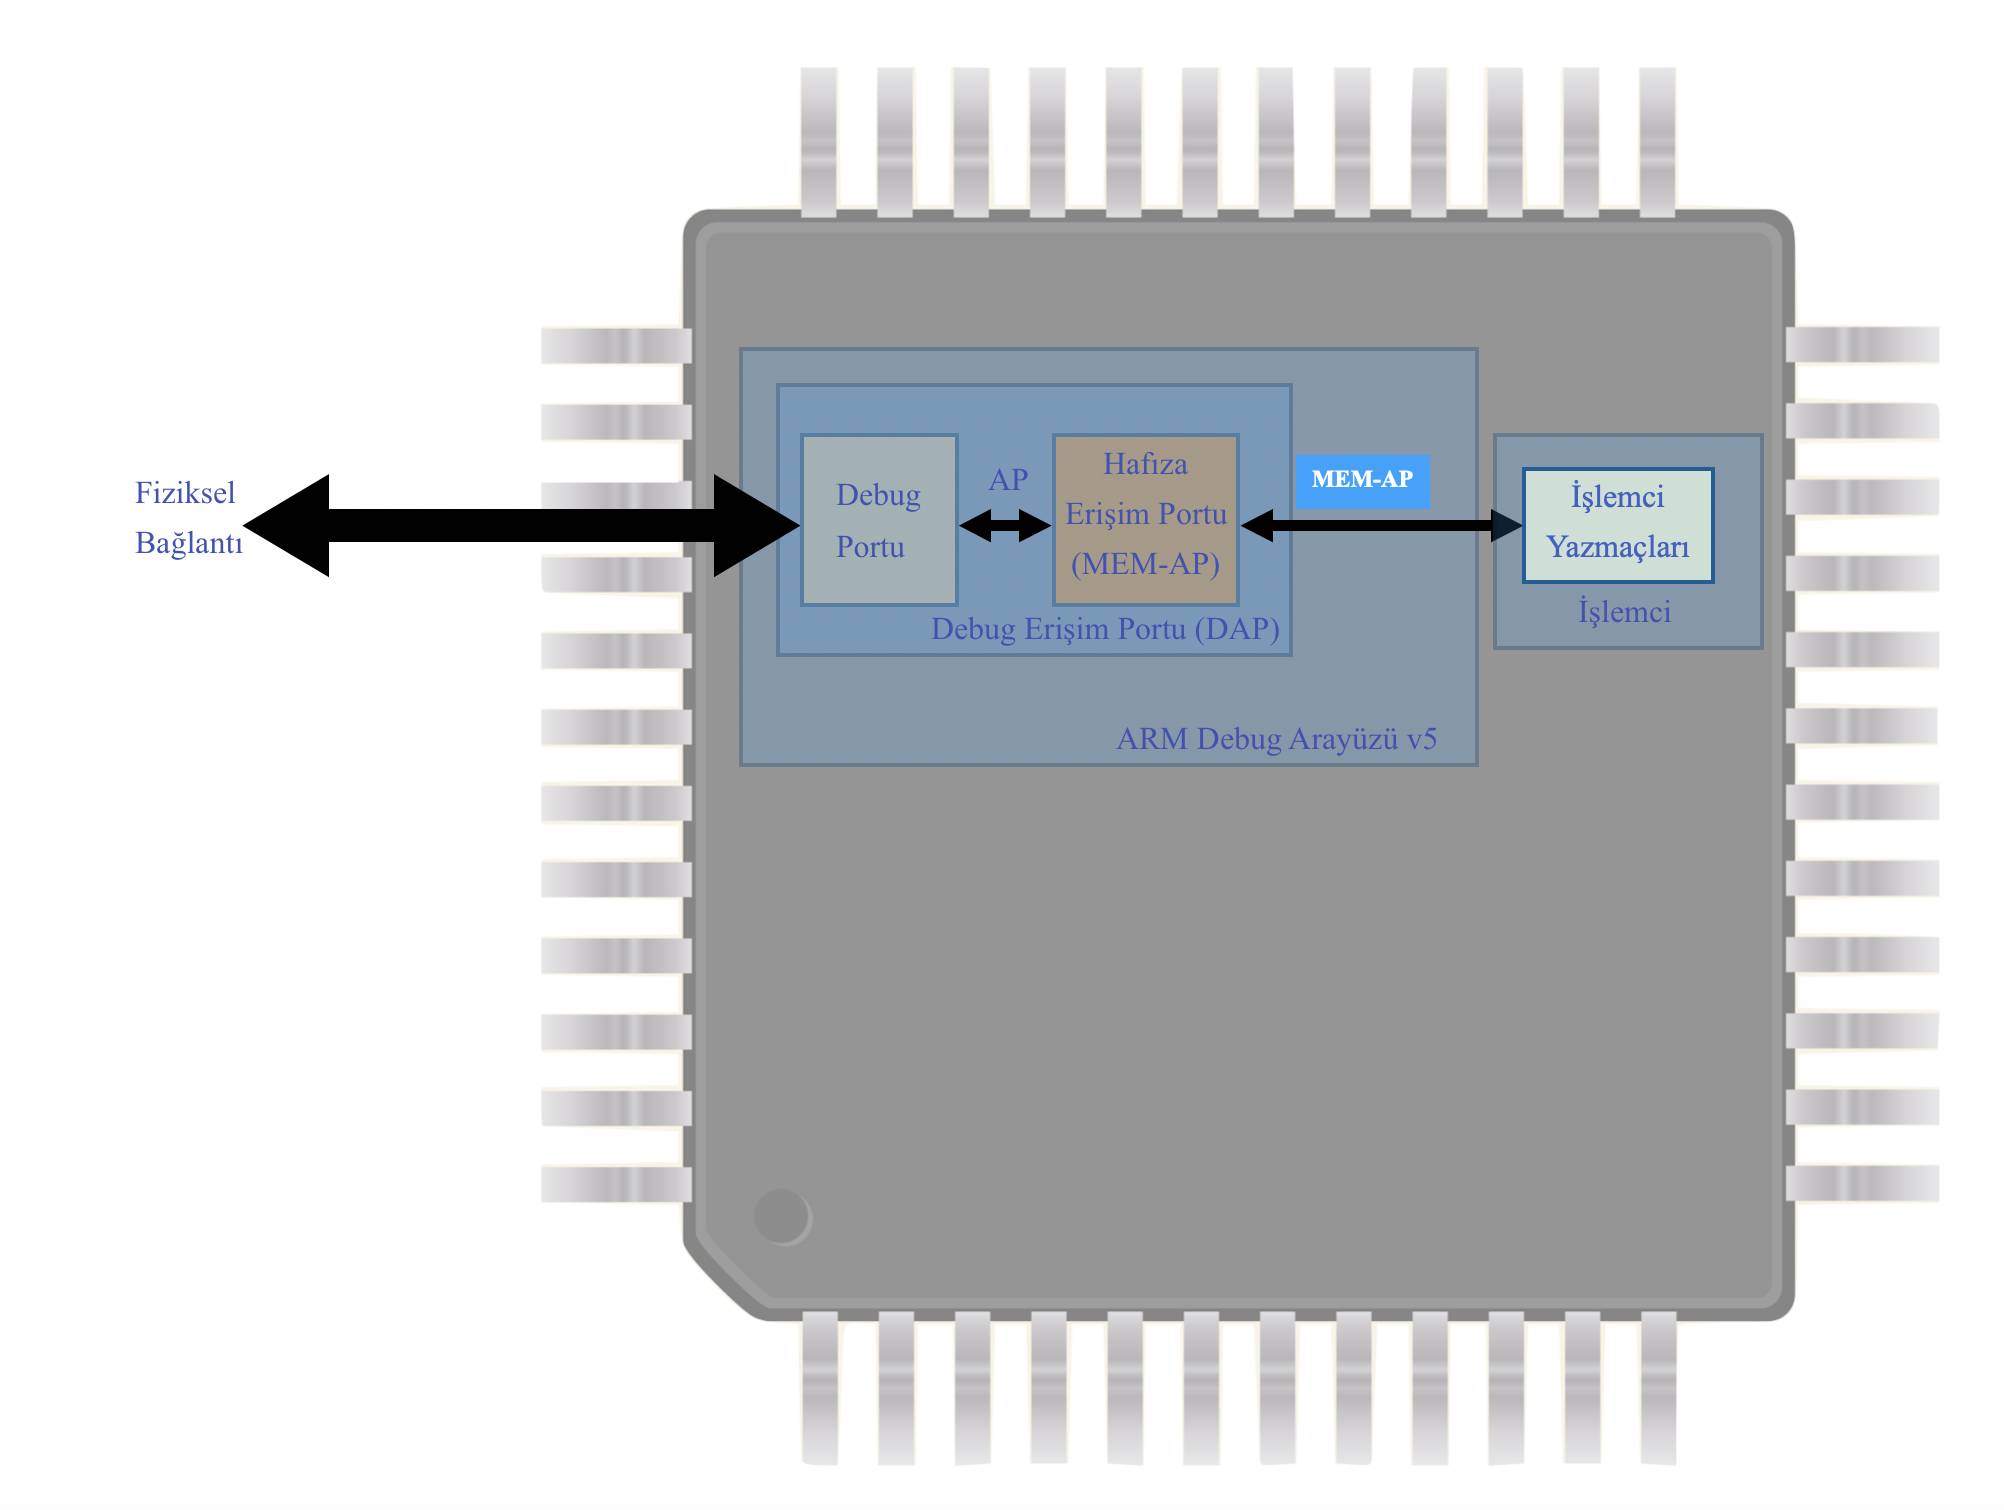
\includegraphics[width=\textwidth]{gorseller/memAp}
\caption{ARM Hata Ayıklama Portu}\label{fig:memAp}
\end{figure}

\section{SWD Protokolü}

SWD protokülü iki pin üzerinden (SWDIO-SCLK) hedef işlemcinin hata ayıklama portuna erişim sağlamaktadır. SWD'nin kullandığı iki pinden birisi olan SWDIO pini iki yönlü hat olup
veri alış-verişinin yapıldığı veri hattır. Diğer pin olan (SCLK), iletişim için gerekli olan saat (clock) sinyalini barındıran sinyal hattıdır. Saat sinyali hattı servis sunucusu tarafından sağlanır.

\section{SWD Bağlantı ve Reset (Line Reset)}

Hedef cihazın Hata Ayıklama Portu'na fiziksel olarak bağlanıldıktan sonra, SWDIO pini lojik 1 seviyesine çekilerek SCLK hattından en az 50 puls verilmelidir. Bu işleme hat sıfırlama (Line Reset) adı verilir.
ARM işlemcisinide bulunan SWD Hata Ayıklama portunu seçmek için hat sıfırlama işleminden sonra onaltı bitlik "0xE79E" verisi, veri hattından saat sinyali ile birlikte gönderilir. Ardından
işlemcinin 'IDCODE' yazmacı okunur. Eğer okunan yazmaç değeri doğru ise SWD protoklü başarılı bir şekilde başlamış demektir.

\section{Veri Gönderme ve Alma Süreçleri}

SWD protokolü 3 farklı fazdan meydana gelmektedir. Bunlar;
\begin{itemize}
	\item İstek Fazı: Servis Sunucusu 8 bitlik istek paketini hedef cihaza gönderir.
	\item Doğrulama Fazı: Hedef cihaz 3 bitlik doğrulama kodunu servis sunucusuna gönderir.
	\item Veri Fazı: İstek fazında bulunan okuma-yazma isteğine bağlı olarak hedef cihaz yada sunucu cihaz 33 bitlik veriyi veri hattından gönderir.
\end{itemize}


\begin{figure}[h]
\centering
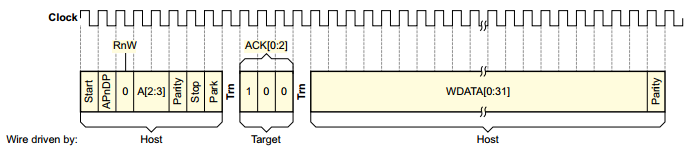
\includegraphics[width=\textwidth]{gorseller/swd}
\caption{SWD Veri Göndeme Alma Süreçleri}\label{fig:swdPhase}
\end{figure}

\subsection{İstek Fazı}

İstek Fazı 8 bitlik veriden oluşmaktadır ve sunucu cihaz tarafından hedef cihaza gönderilir. Bu verinin her biti;
\begin{itemize}
	\item \textbf{Start:} Tek bitlik başlangıç biti. Değeri her zaman 1 olmalı.
	\item \textbf{APnDP:} Erişim portu (AP) yada hata ayıklama (DP) portu seçim bitidir. Erişim portu için 1, hata ayıklma portu için 0 olmalıdır.
	\item \textbf{RnW:} Gönderilen isteğin yazma yada okuma isteği olduğunu belirten bittir. Yazma işlemi için 0, okuma işlemi için 1 olmalıdır.
	\item \textbf{A[2:3]} İki bitlik erişim ve hata ayıklama portunun yazmaç adresini barındırır.
	\item \textbf{Parity:} ApnDp, RnW ve A[2:3] bitlerinden oluştulmuş teklik-çiftlik kontrol bitidir. Tek sayı için 0, çift sayı için 1 olmadır.
	\item \textbf{Stop:} Tek bitlik bitiş bitini belirtir. Her zaman 0 olmadır.
	\item \textbf{Park:} Tek bitlik park biti. Her zaman 1 olmalıdır.
\end{itemize}

\begin{figure}[h]
\centering
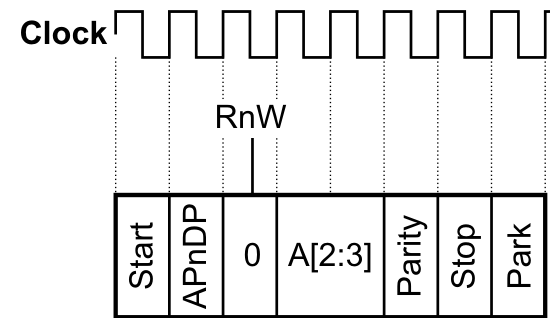
\includegraphics[width=\textwidth]{gorseller/dataPhase}
\caption{SWD İstek Fazı}\label{fig:dataPhase}
\end{figure}

\subsection{Doğrulama Fazı}
ACK fazı (Acknowledge phase) üç bitlik \acrfull{LSB} öncelikli, istek fazında gönderilen isteğe karşılık olarak hedef cihazın cevabını belirten veri fazıdır.
Üç farklı ACK cevabı vardır. Bunlar;
\begin{itemize}
	\item \textbf{OK:} Başarılı operasyonu belirtir. Hedef cihazın isteği doğru bir şekilde aldığını ve sistemin uygun olduğunu belirtir. Cevap olarak "0b001" sayını gönderir.
	\item \textbf{WAIT:} Hedef cihazın istek için hazır olmadığını ve daha sonra tekrar denenmesini belirten cevaptır. Cevap olarak "0b010" sayısını gönderir.
	\item \textbf{FAULT:} İstek sonucunda bir hata olduğunu belirtir. Değeri; "0b100" olarak belirtilir.
\end{itemize}

\subsection{Veri Fazı}

Veri fazında, istek doğrultusunda hedef cihazdan sunucuya yada sunucu cihazdan hedef cihaza gönderilen 33 bitlik veriyi içerir. Bu verinin 32 biti veriyi, 33. biti ise teklik-çiftlik doğrulama biti olarak tanımlanır.

\subsection{Veri Hattı Yön Değişim Periyodu (Turnaround Period-Trn)}

SWDIO veri hattının çift yönlü olduğunu belirtmiştik. Her istek fazından sonra ve isteğe bağlı olarak veri hattının yönü değişmesi gerekiyor. Bu yön değişimini sunucu cihaz tarafında, faz sonunda hattın yönünün değiştiğini belirtir.
Bu değişim istek fazı ile doğrulama fazı arasıdan ve veri fazında yazma işlemi varsa yön değişim periyodu uygulanır.

\section{SW-DP Yazmaçları}

SWD ile bağantı kurduğumuz Seri Hat Hata Ayıklama Portunun yazmaçları Tablo \ref{tab:SwDpReg} verilmiştir. Yazmaç adresleri okuma yada yazma isteğine bağlı olarak, aynı adresler farklı yazmaçlara karşılık gelebilir.
\begin{table}[h]
\centering
\caption{SW-DP Yazmaç Adresleri.}\label{tab:SwDpReg}
\begin{tabular}{|l|l|l|}
	\hline
	Adres	& Okuma	& Yazma \\ \hline
	0x00	& IDCOE & ABORT \\ \hline
	0x04	& CTRL/STAT & CTRL/STAT \\ \hline
	0x08	& RESEND & SELECT \\ \hline
	0x0C	& RDBUFF & N/A \\ \hline
\end{tabular}
\end{table}

\section{Hafıza Erişim Portu Yazmaçları (MEM-AP)}

Hafıza erişim portu, bellek alt sistemlerine erişim sağlar. Bellek, çevre birimleri ve hata ayıklama bileşenleri işlemcinin hafıza haritasında tamınlı olduğu için
\acrfull{MEM-AP}, hem işlemcinin programlanmsında hem de hata ayıklamada kullanılır.

\begin{table}[h]
\centering
\caption{MEM-AP Yazmaç Adresleri.}\label{tab:MemApReg}
\begin{tabular}{|l|l|l|l|}
	\hline
	Adres 	& Bank 	& Yazmaç & Açıklama \\ \hline
	0x00 	& 0x00 	& CSW 	& Control/Status Word Yazmacı \\ \hline
	0x04	& 0x00 & TAR 	& Transfer Address Yazmacı \\ \hline
	0x0C	& 0x00 & DRW 	& Data Read/Write Yazmacı \\ \hline
	0xFC	& 0x0F & IDR 	& Identification Yazmacı \\ \hline
\end{tabular}
\end{table}

\subsection{Control/Status Word Yazmacı}

CSW yazmacı \acrshort{MEM-AP} portuna konrol ve konfigürasyon için erişim sağlayan yazmaçtır. Yazmaçta bulunan 32 bitlik verinin sadece 5 bitlik kısmı anlamlıdır. Bunlar Tablo \ref{tab:csw}'de gösterilmiştir.

\begin{table}[h]
\centering
\caption{CSW Yazmacı Anlamlı Bitler ve Açıklamaları}\label{tab:csw}
	\begin{tabular}{|l|l|p{10cm}|}
	\hline
	Bitler  & İşlevi	& Açıklama \\ \hline
	[30:24] & Prot 		& Veri yolu koruma biti olarak tanımlanır. \\ \hline
	[5:4]   & AddrInc 	& Adres verisini otamatik olarak arttırım biti olarak tanımlanır. \\ \hline
	[2:0]   & Size 		& Yazılacak yada okunacak olan verinin boyutunu belirtir;

	"0b000": 8 bit; "0b001": 16 bit; "0b010": 32 bit \\ \hline

\end{tabular}
\end{table}

\subsection{TAR Yazmacı}

TAR yazmacı okuma yada yazma için erişilecek olan hafıza adresini tutar. Eğer CSW yazmacının AddrInc bitleri "0b01" olarak setlenmiş ise
DRW yazmacına başarılı erişim sağlandıkça otomatik olarak artar.

\subsection{DRW Yazmacı}

DRW yazmacı, TAR yazmacında tutulan adresteki veriyi yada TAR adresine yazılmak için gönderilen veriyi tutmaktadır. Örnek olarak "0x20000000" adresteki veriyi
okumanmak istediğinde, öncelikle TAR yazmacına okunmak istenen adres yazılır, ardından hata ayıklama portu o adresteki veriyi DRW yazmacına aktarır.


\subsection{IDR Yazmacı}

IDR yazmacı, erişim portunun tanımlama kodunu tutar. Örnek olarak, ARM Cortex-M0 tabanlı olan işlemcilerde bu değer "0x0477003" olarak okunur.
